% =====================================================================
%  Per-Window Oracle Headroom Is Not Learnable
%  Elsevier CAS single-column manuscript (cas-sc), prepared for
%  submission to Information Sciences.
%
%  Every number in this file is regenerated from persisted artifacts:
%    monday_final/weekend_report.{md,json}
%    monday_final/paper/audit_strata.csv
%    monday_final/paper/splitfix/*.csv
%    artifacts/robustness/*.csv           (src/robustness.py)
%    paper/tables_robust/*.tex            (tools/make_robustness_tables.py)
%    tools/recompute_main_table.py monday_final/p1_results.csv
%
%  Build:  pdflatex main && bibtex main && pdflatex main && pdflatex main
% =====================================================================
\documentclass[a4paper,fleqn]{cas-sc}

\usepackage[numbers]{natbib}
\usepackage{amsmath,amssymb}
\usepackage{booktabs}
\usepackage{graphicx}

\newtheorem{proposition}{Proposition}
\newproof{pf}{Proof}

\newcommand{\arm}[1]{\texttt{#1}}
\setlength{\tabcolsep}{3.5pt}

% Shrink a table to the text width *only* when it is genuinely too wide.
% A bare \fitwidth{...} also magnifies narrow tables, which
% makes a four-column table print larger than the body text.
\newcommand{\fitwidth}[1]{%
  \resizebox{\ifdim\width>\linewidth \linewidth\else \width\fi}{!}{#1}}

% Corresponding e-mail address. Defined inside a catcode-safe group so that an
% underscore in the local part cannot break the build; edit only this one line.
% \ead detokenises its argument, so the macro must be expanded *before* \ead
% sees it (see \expandafter below) -- otherwise the macro name is typeset.
\begingroup
\catcode`\_=12
\gdef\correspemail{1367489893@qq.com}
\gdef\secondemail{1577027526@qq.com}
\endgroup

\begin{document}
\let\WriteBookmarks\relax
\def\floatpagepagefraction{1}
\def\textpagefraction{.001}

\shorttitle{Per-window oracle headroom is not learnable}
\shortauthors{M. Liu and C. Chen}

\title[mode = title]{Per-window oracle headroom is not learnable:
a feedback-delay audit of plug-in selection for time series forecasting}

\author[1]{Mianhan Liu}[orcid=0009-0000-0274-1062]
\cormark[1]
\expandafter\ead\expandafter{\correspemail}
\credit{Conceptualization, Methodology, Software, Formal analysis,
Investigation, Data curation, Visualization,
Writing -- original draft, Writing -- review \& editing}

\author[1]{Chen Chen}[orcid=0009-0001-1991-9370]
\expandafter\ead\expandafter{\secondemail}
\credit{Validation, Investigation, Writing -- review \& editing}

\affiliation[1]{organization={Independent Researcher},
                city={Shanghai},
                postcode={200000},
                country={China}}

\cortext[1]{Corresponding author.}

\begin{abstract}
Model-agnostic ``plug-and-play'' modules for time series forecasting---instance
normalization, non-stationarity correction, frequency-domain losses---are reported
as helpful, yet their gain flips sign across backbones. The natural response is to
learn \emph{when} to attach \emph{which} module. In $2{,}035$ single-GPU training
runs across four backbones, eight datasets and four horizons, we show that this
research program is empty under the only causally legal deployment setting. First,
the reported effect is smaller than three near-universal reporting choices:
complete-block filtering, the error metric, and mean versus median. Each flips at
least one verdict. Second, the per-window oracle that motivates gating is provably
invariant to re-labeling which arm produced which error, so its $+10.15\%$
headroom is no evidence of learnability; a seed-paired replication nevertheless
shows the structure is real, with $79\%$ surviving a seed change. Third, the
decisive quantity is the correlation length of best-arm identity: its median
half-life is $5.1\%$ of the forecast horizon, whereas deployment forces a
one-horizon decision lag. Three selector families accordingly lose to the arm
frozen on validation, and the one legal axis, lead time, yields only $+0.24\%$.
Only a constant mis-selection is recoverable. We distill the audit into a
checklist for adaptive-selection claims.
\end{abstract}

\begin{highlights}
\item Block filtering flips a plug-in verdict from significant to null.
\item Metric and mean-vs-median choices each flip a second verdict.
\item Per-window oracle headroom survives per-window arm relabeling.
\item Best-arm identity has a median half-life of 5.1\% of the forecast horizon.
\item The one causally legal axis, lead time, has 0.24\% oracle headroom.
\end{highlights}

\begin{keywords}
time series forecasting \sep model selection \sep delayed feedback \sep
benchmarking \sep reproducibility \sep negative result
\end{keywords}

\maketitle

\section{Introduction}

The past five years have produced a steady stream of \emph{model-agnostic}
additions to deep time series forecasters: reversible instance
normalization~\cite{revin}, explicit non-stationarity correction~\cite{san},
channel clustering~\cite{ccm}, frequency-domain training objectives~\cite{fredf}. Each is
presented as an orthogonal, architecture-independent, essentially free
improvement. Two facts sit uneasily beside that framing.

First, benchmarks have saturated. On ETT / Electricity / Weather, the annual
improvement of the best published model has fallen from double digits to a few
percent, and unified re-evaluations attribute much of the remaining spread to
pipeline details rather than to the method itself~\cite{tfb,champions}; in that
regime a reported $+0.3\%$ is indistinguishable from a reporting choice.

Second, the sign of the gain is unstable. Practitioners who attach the same
plug-in to a linear model and to a patch transformer routinely observe gains of
opposite sign. If the gain is conditional, the useful engineering artifact is not
another plug-in but a \emph{decision rule}: given (backbone, dataset, horizon), or
even given the current window, decide whether to attach a plug-in and which one.

This paper is a systematic, negative, and --- we argue --- \emph{mechanistic}
answer to that decision problem. We do not propose a new plug-in. We build the
full conditional-gain matrix, quantify how much of the reported effect is
produced by reporting conventions rather than by the method, attack the decision
problem with three independent selector families, and finally explain the uniform
failure with a single quantitative mechanism: \textbf{the correlation length of
best-arm identity is one to two orders of magnitude shorter than the feedback
delay that deployment imposes}.

Our contributions are fourfold.
\begin{enumerate}\itemsep2pt
\item \textbf{Three reporting levers, each larger than the effect.} Complete-block
filtering of the main table, the choice of error metric, and the choice between a
mean and a median each move the headline by more than the effect being claimed,
and each flips at least one plug-in verdict (\S\ref{sec:main}). A fourth,
reporting a plug-in only at its published default hyper-parameter, accounts for
essentially all of one plug-in's apparent benefit (\S\ref{sec:tuning}).
\item \textbf{Effect size in interpretable units.} We put the block-level
plug-in effect on the same scale as the run-to-run noise of a training seed and
as the compute it costs (\S\ref{sec:effectsize}): $28\%$ of block-level effects
are smaller than same-configuration seed noise, and the arm with the largest
compute overhead is also the only one that is significantly \emph{worse} than
doing nothing.
\item \textbf{An impossibility-style audit.} We prove and empirically verify
that the per-window oracle used to motivate gating is invariant to per-window
arm re-labeling (\S\ref{sec:oracle}), then measure the quantity that actually
governs learnability --- the lagged predictability of best-arm identity --- and
show it decays to chance well before the legal decision lag
(\S\ref{sec:halflife}). A seed-paired replication rules out the trivial
explanation that the headroom is training noise (\S\ref{sec:seed}).
\item \textbf{A falsified-hypotheses table, and a closed loop.} Three selector
families and two control conditions, all evaluated on identical decision groups
against a deployable baseline, are all negative, with a delay sweep pinning the
break-even point at $0.25\times H$ (\S\ref{sec:selectors}). Crucially, we also
audit the one selection axis that is \emph{not} subject to feedback delay, namely
the lead-time index within a forecast (\S\ref{sec:leadtime}); its oracle is worth
only $+0.24\%$. Both axes are therefore closed, for two different reasons.
\end{enumerate}

We deliberately report the deployable baseline
\arm{best\_fixed\_val} --- the arm chosen on validation data and then frozen ---
rather than the post-hoc best arm. Much of the apparent success of adaptive
selection in the literature disappears against this baseline, and
\S\ref{sec:recover} shows that what remains is a validation$\to$test transfer
effect, not adaptation.

\section{Related work and positioning}

\textbf{Plug-in modules.} Reversible instance normalization~\cite{revin} removes
instance-level distribution shift by de-normalizing the output with the input
statistics. Non-stationarity correction methods~\cite{san} estimate slice-wise
statistics and extrapolate them; we implement a \emph{training-free surrogate}
(\arm{san\_lite}, EWMA extrapolation of slice statistics) so that the arm adds
zero trainable parameters and zero per-dataset hyper-parameters, and we label it
as a surrogate throughout rather than claiming to reproduce~\cite{san}.
Frequency-domain losses~\cite{fredf} (\arm{fredf}) add a spectral term with
weight $\alpha$. Our contribution to this literature is not a new member but an
audit of how their gains are reported.

\textbf{Benchmark-hygiene work.} A line of work has shown that apparent
progress in long-horizon forecasting is sensitive to pipeline details such as
\texttt{drop\_last}, look-back length and checkpoint selection, and that
conclusions change once evaluation is unified~\cite{tfb,tslib,dlinear}; a recent
reproducible re-evaluation of eight models on fourteen datasets reports that
small changes to the experimental setup or to the evaluation metric are enough
to overturn claimed state-of-the-art results~\cite{champions}. We re-run every
baseline ourselves under one fixed
protocol for exactly this reason and never copy numbers across papers.
Section~\ref{sec:main} adds new items to that list: which \emph{blocks} enter the
aggregate, which \emph{metric} is reported, and which \emph{central estimator} is
used are each a significance lever, and we follow~\cite{demsar} on how
block-level comparisons should be tested.

\textbf{Adaptive / online model selection.} Expert-advice and bandit selection
over forecasters is classical~\cite{cesabianchi}, and dynamic
expert-arbitration for time series is an established
family~\cite{arbitrage}, as is drift-triggered adaptation~\cite{gama}. The
regret guarantees, however, assume feedback arrives shortly after the decision;
delayed-feedback online learning quantifies the degradation when it does
not~\cite{joulani}. The novelty here is empirical and negative: in
$H$-step-ahead forecasting the feedback delay is \emph{structurally} $H$
windows, and we measure the identity correlation length that this delay must be
compared against. To our knowledge the ratio
$\text{half-life}/H$ has not previously been measured for plug-in selection;
it is the quantity that decides the problem.

\section{Protocol}
\label{sec:protocol}

\paragraph{Grid.}
Backbones: \arm{DLinear}~\cite{dlinear}, \arm{PatchTST}~\cite{patchtst},
\arm{TimesNet}~\cite{timesnet}, \arm{iTransformer}~\cite{itrans}
(imported unmodified from a standard library~\cite{tslib}; we do not use its
training script). Datasets: ETTh1, ETTh2, ETTm1, ETTm2, Electricity, Exchange,
Weather (horizons $96/192/336/720$, look-back $96$) and ILI (horizons
$24/36/48/60$, look-back $36$). Arms: \arm{none}, \arm{revin}~\cite{revin},
\arm{san\_lite} (surrogate for~\cite{san}), \arm{fredf}~\cite{fredf}
($\alpha{=}0.5$), plus an $\alpha$-sweep pool
$\alpha\in\{0.1,0.3,0.5,0.7,0.9\}$ on the plain objective and
$\alpha\in\{0.1,0.5,0.9\}$ on the $\sqrt{H}$-normalized one
(\S\ref{sec:tuning}).

\paragraph{Three phases.}
Phase~1 is the main gain matrix: $844/844$ cells. Phase~2 persists per-window
squared errors on validation and test for the nominal four-arm pool:
$423/428$ cells ($5$ missing cells are all \arm{TimesNet}$\times H{=}720$).
Phase~3 is the $\alpha$ sweep over three backbones (\arm{TimesNet} excluded):
$768/768$ cells, i.e.\ $96$ blocks $\times$ $8$ arms (seven $\alpha$ settings
plus a re-trained \arm{none} control). In total we perform $2{,}035$ training
runs on a single V100 GPU, in fp32 with AMP enabled on the largest datasets. The
three phases overlap by design ($2{,}035$ counts runs, not
distinct configurations: phase~1 includes $3$ seeds on a subset, and phase~2
re-runs the four-arm pool to persist per-window traces).

\paragraph{Statistical block.}
A block is a (dataset $\times$ horizon $\times$ backbone) triple, not a dataset.
This choice is not cosmetic. With $k{=}4$ methods and only the $N{=}8$ datasets
as blocks --- the aggregation level most plug-in papers use --- the Nemenyi
critical difference is $1.66$, wider than the entire observed rank range, so no
ranking can be significant at that resolution. At our $N{=}128$ blocks it falls
to $0.41$. We follow~\cite{demsar}
for the Friedman/Nemenyi machinery, and all paired tests are Wilcoxon
signed-rank reported both raw and with Holm correction inside an explicitly
declared family.

\paragraph{A documented \arm{revin} pruning.}
\arm{PatchTST}, \arm{TimesNet} and \arm{iTransformer} hard-code their own
instance normalization, so wrapping them in an external RevIN is mathematically
an approximate identity. We therefore pruned that combination \emph{a priori}
(skip rule \texttt{revin\_on\_internal\_norm\_backbones} in
\texttt{configs/matrix.yaml}) and kept a verification subset ---
$\{$ETTh1, Weather$\}\times\{96,720\}$ on all three backbones, $12$ cells --- to
check the prediction instead of assuming it. It holds: the median gain over
\arm{none} on those $12$ cells is $+0.00\%$ (Wilcoxon $p{=}0.23$), and on
\arm{PatchTST} and \arm{iTransformer} the test MSE is unchanged to four decimals
in $7$ of $8$ cells; the only two cells with a visible effect are \arm{TimesNet}
at $H{=}720$ ($+0.62\%$ and $+5.56\%$). On \arm{DLinear}, which has no internal
normalization, the same arm has a median gain of $+0.98\%$ over $64$ cells. No
cell of the matrix failed to train --- all $844$ phase-1 runs report status
\texttt{ok} --- so every \arm{revin} absence below is this design decision, not
an outage. The consequence for \S\ref{sec:main} is mechanical but must be
stated: because \arm{revin} exists on $44$ blocks by construction,
complete-block filtering over four arms can only ever return those $44$ blocks.

\paragraph{Decision group.}
For window-level analysis a \emph{decision group} is a
(backbone, dataset, horizon) triple for which all arms have aligned per-window
error vectors on the same evaluation windows. We have $127$ groups for test-side
audits. For protocols that must \emph{train} a gate on validation windows we
require a provenance marker certifying deterministic loader order
(\S\ref{sec:threats}); $96$ groups qualify. The nominal pool has four arms, but
under the pruning above the \emph{realized} arm count per group is $4$ in $43$
groups, $3$ in $83$ and $2$ in $1$ (for the $96$
gating groups: $40$ and $56$). Since oracle headroom grows with the number of
arms, we report the realized counts wherever a headroom figure appears and never
pool groups of different sizes into a single headroom claim without saying so.

\paragraph{Baselines.} \arm{none}; \arm{best\_fixed\_val}, the arm with lowest
validation MSE, frozen over the test segment (this is the deployable strong
baseline and the reference for every gain we report); \arm{best\_fixed\_test},
the post-hoc constant arm (an upper bound on any non-time-varying policy); and
the per-window \arm{oracle}.

\section{How the gain is reported: three significance levers}
\label{sec:main}

\subsection{Lever 1: which blocks enter the aggregate}

The standard way to aggregate a plug-in comparison is to keep the blocks in
which \emph{all} arms are available and run a paired test on that subset.
Absent cells, however, are never absent at random. Whatever prunes a cell ---
an out-of-budget corner (heavy backbone $\times$ long horizon $\times$ large
dataset), a crash, or, as here, an explicit design rule --- is correlated with
the very axes along which the plug-in's effect varies. In our matrix, $128$
blocks exist, but only $44$ are complete across four arms, because the
\arm{revin} pruning of \S\ref{sec:protocol} decides the subset; $32$ of those
$44$ ($73\%$) come from \arm{DLinear}, the one backbone without internal
normalization, which is also the backbone on which frequency-domain losses
happen to help most. The filter is therefore a backbone filter wearing a
completeness costume, and the arm it silently re-weights is not the arm that
caused the pruning.

Table~\ref{tab:main} contrasts the two conventions. Pairwise dropping (each
arm compared to \arm{none} on every block where \emph{that pair} exists) is the
correct estimator; complete-block filtering is what the literature does.

\begin{table}[t]
\centering\small
\caption{Same raw runs, two aggregation conventions. Mean relative gain over
\arm{none} (\%), Wilcoxon signed-rank $p$ raw and Holm-adjusted within the family
of three arms (each convention is its own family). The significance flip is not
an artifact of multiplicity: after Holm correction the complete-block convention
still calls \arm{fredf} significant ($0.017$) while the correct pairwise
convention does not ($0.76$).}
\label{tab:main}
\fitwidth{%
\begin{tabular}{llrrrr}
\toprule
Convention & Arm & $N$ & mean & $p$ & $p_\text{Holm}$ \\
\midrule
complete-block ($44$) & \arm{fredf}    & 44  & $+3.60$ & $0.0058$ & $0.017$ \\
\textbf{pairwise}     & \arm{fredf}    & 128 & $\mathbf{-2.37}$ & $0.44$ & $\mathbf{0.76}$ \\
\addlinespace
complete-block ($44$) & \arm{san\_lite}& 44  & $-1.29$ & $0.056$ & $0.11$ \\
\textbf{pairwise}     & \arm{san\_lite}& 128 & $\mathbf{-3.94}$ & $5\!\times\!10^{-8}$ & $\mathbf{1.5\!\times\!10^{-7}}$ \\
\addlinespace
complete-block ($44$) & \arm{revin}    & 44  & $+3.55$ & $0.38$ & $0.38$ \\
pairwise              & \arm{revin}    & 44  & $+3.55$ & $0.38$ & $0.76$ \\
\bottomrule
\end{tabular}}
\end{table}

The direction of the error is not benign. For \arm{fredf} the filter converts a
non-significant negative mean into a significant positive one; for
\arm{san\_lite} it hides a real, strongly significant degradation. On the
complete-block subset a Friedman test rejects
($\chi^2{=}30.9$, $p{=}8.9\!\times\!10^{-7}$, $\mathrm{CD}{=}0.71$) with mean
ranks $\arm{fredf}\,1.93 < \arm{revin}\,2.14 < \arm{none}\,2.59 <
\arm{san\_lite}\,3.34$ --- a clean-looking ranking produced by a subset that is
$73\%$ one backbone.

\begin{table}[t]
\centering\small
\caption{\arm{fredf} vs.\ \arm{none} per backbone, all pairable blocks. The sign
flips and the magnitude spans $21$ points. $p_\text{Holm}$ is adjusted within the
family of four strata; the two significant cells have opposite signs.}
\label{tab:cond}
\begin{tabular}{lrrrr}
\toprule
Backbone & $N$ & mean (\%) & $p$ & $p_\text{Holm}$ \\
\midrule
\arm{DLinear}      & 32 & $+4.56$  & $0.0036$ & $0.011$ \\
\arm{PatchTST}     & 32 & $-16.63$ & $3.3\!\times\!10^{-9}$ & $1.3\!\times\!10^{-8}$ \\
\arm{TimesNet}     & 32 & $+1.41$  & $0.15$ & $0.31$ \\
\arm{iTransformer} & 32 & $+1.17$  & $0.26$ & $0.31$ \\
\bottomrule
\end{tabular}
\end{table}

Table~\ref{tab:cond} shows why the aggregate is so fragile: conditioned on the
backbone, the same plug-in ranges from $+4.6\%$ to $-16.6\%$. \emph{Plug-in
gains are strongly backbone-conditional}, which is the empirical premise that
makes a selection rule attractive in the first place. The rest of the paper
tests whether that premise can be converted into a deployable decision.

\subsection{Lever 2: which error metric is reported}

Every number above is MSE, as is standard. Because our evaluation accumulates
MAE in the same forward pass, re-running the entire test on MAE costs nothing,
and the outcome is not a formality (Table~\ref{tab:metric-robust}). The verdict
for \arm{revin} \emph{flips}: it is indistinguishable from \arm{none} on MSE
(median $+0.03\%$, $p_\text{Holm}{=}0.76$) and significantly better on MAE
(median $+1.38\%$, $p_\text{Holm}{=}1.4\!\times\!10^{-5}$, winning $37$ of $44$
blocks). The flip is not a ranking artifact: the per-block gains on the two
metrics correlate at Spearman $\rho{=}0.64$ but agree in sign in only $64\%$ of
blocks, i.e.\ \arm{revin} shifts the error distribution in a way that a squared
loss and an absolute loss genuinely disagree about. This is the expected
signature of a normalization module: it trims many moderate errors while
occasionally enlarging a few large ones, which MAE rewards and MSE does not.
For \arm{fredf} and \arm{san\_lite} the two metrics agree
($\rho{=}0.97$ and $0.84$).

\begin{table}[t]
\centering
\caption{Metric robustness of the plug-in verdicts.}\label{tab:metric-robust}
\fitwidth{%
\begin{tabular}{llrccccrcl}
\toprule
Arm & Metric & $N$ & W/T/L & Median gain (\%) & 95\% CI & $p$ & $p_{\text{Holm}}$ & $r$ & Verdict \\
\midrule
\texttt{revin} & MSE & 44 & 23/0/21 & +0.03 & [-0.52, +0.84] & 0.382 & 0.764 & 0.13 & n.s. (better) \\
 & MAE & 44 & 37/0/7 & +1.38 & [+0.43, +4.05] & $4.8\!\times\!10^{-6}$ & $1.4\!\times\!10^{-5}$ & 0.65 & \textbf{sig.} (better) \\
\multicolumn{10}{l}{\quad\footnotesize cross-metric: Spearman $\rho=0.64$, sign agreement $64\%$, verdict \textbf{flips}} \\
\addlinespace[2pt]
\texttt{san\_lite} & MSE & 128 & 30/0/98 & -3.01 & [-4.35, -2.05] & $4.9\!\times\!10^{-8}$ & $1.5\!\times\!10^{-7}$ & 0.48 & \textbf{sig.} (worse) \\
 & MAE & 128 & 44/0/84 & -1.01 & [-1.60, -0.65] & $8.7\!\times\!10^{-4}$ & 0.002 & 0.29 & \textbf{sig.} (worse) \\
\multicolumn{10}{l}{\quad\footnotesize cross-metric: Spearman $\rho=0.84$, sign agreement $84\%$, verdict consistent} \\
\addlinespace[2pt]
\texttt{fredf} & MSE & 128 & 70/0/58 & +0.45 & [-0.45, +1.27] & 0.438 & 0.764 & 0.07 & n.s. (better) \\
 & MAE & 128 & 79/0/49 & +0.90 & [+0.41, +1.57] & 0.323 & 0.323 & 0.09 & n.s. (better) \\
\multicolumn{10}{l}{\quad\footnotesize cross-metric: Spearman $\rho=0.97$, sign agreement $93\%$, verdict consistent} \\
\addlinespace[2pt]
\bottomrule
\end{tabular}}
\vspace{3pt}\parbox{\linewidth}{\footnotesize Paired Wilcoxon signed-rank per arm against \texttt{none}; blocks are (dataset $\times$ horizon $\times$ backbone), matched pairwise so that one arm's pruning cannot shrink another arm's sample. Holm correction is applied within each metric (family size 3). CIs are percentile bootstrap over blocks ($10^4$ resamples, blocks resampled jointly to preserve pairing). Positive gain $=$ lower error than \texttt{none}.}
\end{table}


\subsection{Lever 3: mean or median, and the tail that hides behind it}

A third choice is left implicit almost everywhere: papers report a \emph{mean}
relative gain and test it with a \emph{rank} test. The two target different
functionals, and on this data they disagree about whether a plug-in works at all
(Table~\ref{tab:estimator-lever}). For \arm{fredf} the mean is $-2.37\%$ while
the median is $+0.45\%$, and the same conflict appears on MAE ($-1.18\%$ vs.\
$+0.90\%$). Neither number is wrong; they answer different questions, and a
paper that prints the mean while testing the median is not testing what it
reports.

The mechanism is a heavy left tail (skew $-4.5$), and the tail is not diffuse: it
is one identifiable corner of the grid. \arm{fredf} degrades
\texttt{Electricity} with \arm{PatchTST} by $-31\%$, $-61\%$, $-96\%$ and
$-123\%$ at $H{=}96,192,336,720$, i.e.\ the failure grows monotonically with the
horizon, while the same plug-in helps \arm{DLinear} at $H{=}720$ by $+19\%$ on
\texttt{ETTm2} and $+25\%$ on \texttt{Exchange}. Overall $10.9\%$ of blocks are
more than $10\%$ worse than \arm{none} and $3.9\%$ are more than $25\%$ worse.
Reporting a median alone would sell \arm{fredf} as a small free win; reporting a
mean alone would sell it as harmful; reporting either alone hides a deployment
risk that a practitioner needs to know about. \arm{san\_lite} carries the highest
frequency of moderate damage ($21.9\%$ of blocks below $-10\%$) but its worst
case is milder ($-30\%$).

\begin{table}[t]
\centering
\caption{The choice of central estimator is a third significance lever.}\label{tab:estimator-lever}
\fitwidth{%
\begin{tabular}{llrrrrrrlr}
\toprule
Arm & Metric & Mean (\%) & Median (\%) & Mean$-$Med & Skew & $<\!-10\%$ & $<\!-25\%$ & Worst block & Worst (\%) \\
\midrule
\texttt{revin} & MSE & +3.55 & +0.03 & +3.52 & +2.19 & 2.3\% & 0.0\% & \footnotesize\texttt{Exchange/720/DLinear} & -14.1 \\
 & MAE & +5.01 & +1.38 & +3.63 & +1.57 & 0.0\% & 0.0\% & \footnotesize\texttt{ETTh1/720/TimesNet} & -5.9 \\
\addlinespace[2pt]
\texttt{san\_lite} & MSE & -3.94 & -3.01 & -0.93 & +0.96 & 21.9\% & 2.3\% & \footnotesize\texttt{ILI/36/TimesNet} & -30.0 \\
 & MAE & -1.08 & -1.01 & -0.07 & +1.12 & 7.8\% & 0.0\% & \footnotesize\texttt{ILI/60/TimesNet} & -19.4 \\
\addlinespace[2pt]
\texttt{fredf} & MSE & \textbf{-2.37} & \textbf{+0.45} & -2.82 & -4.47 & 10.9\% & 3.9\% & \footnotesize\texttt{Electricity/720/PatchTST} & -123.4 \\
 & MAE & \textbf{-1.18} & \textbf{+0.90} & -2.07 & -4.60 & 6.2\% & 3.1\% & \footnotesize\texttt{Electricity/720/PatchTST} & -80.0 \\
\addlinespace[2pt]
\bottomrule
\end{tabular}}
\vspace{3pt}\parbox{\linewidth}{\footnotesize All columns are computed on the \emph{same} pairwise-matched blocks as Table~\ref{tab:metric-robust}; only the summary functional changes. Bold rows are sign conflicts, where the mean and the median disagree on whether the plug-in helps at all. ``$<\!-10\%$'' is the fraction of blocks whose error is more than $10\%$ worse than \texttt{none}. A paired Wilcoxon test targets the median, so a paper that reports a mean and tests with Wilcoxon is not testing the quantity it reports.}
\end{table}


We therefore report median, mean, a paired bootstrap interval and the tail
fractions together for every arm, and we recommend the same in
\S\ref{sec:checklist}. Note that the three levers are independent: they act on
which blocks are counted, which loss is measured, and how the counted blocks are
summarized, so a paper can be internally consistent and still be off by more
than its own effect size on all three at once.

\section{How the gain is tuned: ``plug-and-play'' is a tuning effect}
\label{sec:tuning}

Frequency-domain losses introduce one hyper-parameter, the spectral weight
$\alpha$, and are reported at a fixed default. We sweep
$\alpha\in\{0.1,0.3,0.5,0.7,0.9\}$ on the plain objective and
$\alpha\in\{0.1,0.5,0.9\}$ on the $\sqrt{H}$-normalized one, giving
$96\times(5+3)=768$ $\alpha$-cells for analysis. Of these, the $96$ plain
$\alpha{=}0.5$ cells are the phase-1/2 reference and the remaining $672$ are
trained in phase~3; phase~3's own run count is also $768$ because it re-trains
its own \arm{none} control ($96\times(7\ \alpha\text{ settings}+1)$), so the two
$768$s count different things and are not a duplicate.
The $96$ blocks are $3$ backbones $\times$ $8$ datasets $\times$ $4$ horizons ---
\arm{TimesNet} is excluded from the sweep for cost reasons, so this section does
not claim to cover it.

\begin{table}[t]
\centering\small
\caption{The apparent benefit of a frequency-domain loss is recovered by
per-cell tuning of its one hyper-parameter; at the published default the arm is
harmful. $96$ blocks, three backbones (\arm{TimesNet} excluded).}
\label{tab:alpha}
\fitwidth{%
\begin{tabular}{lr}
\toprule
Setting & mean gain (\%) \\
\midrule
fixed $\alpha{=}0.5$ (published default) & $-3.70$ \\
per-cell $\alpha$ tuned on \emph{validation} & $+1.79$ \\
per-cell $\alpha$ tuned on \emph{test} (cheating bound) & $+2.29$ \\
\midrule
\textbf{tuning gap} & $\mathbf{+5.48}$ \\
best \emph{single} $\alpha$ chosen on validation ($\alpha{=}0.1$) & $+0.12$ \\
\quad with $\sqrt{H}$ normalization ($\alpha{=}0.1$) & $+0.18$ \\
\bottomrule
\end{tabular}}
\end{table}

Two readings follow from Table~\ref{tab:alpha}. (a) The method is not
plug-and-play: essentially all of its benefit is recovered by per-cell tuning,
and $59.4\%$ of blocks are positive only after tuning. (b) The tuning is
genuinely per-cell: no single $\alpha$ transfers ($+0.12\%$), and the number of
distinct optimal $\alpha$ values that one (backbone, dataset) pair takes across
horizons is $1.79$. Normalizing $\alpha$ by $\sqrt{H}$ reduces that to $1.42$
and adds $0.06$ points --- we report it as an ablation line, not as a
contribution.

The gap between validation-tuned ($+1.79$) and test-tuned ($+2.29$) is only
$0.5$ points, so honest tuning is nearly as good as cheating; the problem is not
selection noise, it is that the default is wrong for most cells.

\section{How big the gain is: seed noise and compute cost}
\label{sec:effectsize}

Before asking whether a selector can exploit these gains, it is worth asking how
large they are in units a practitioner can act on. Two cheap references
make the effect size interpretable, and both are computable from artifacts we
already have (Table~\ref{tab:seed-cost}).

\paragraph{Against seed noise.}
For $208$ configurations we trained three seeds, giving $144$ block--arm pairs in
which both the arm and \arm{none} have a within-configuration standard
deviation. We compare the plug-in effect against
$\sigma_\text{seed}=\sqrt{s^2_\text{arm}+s^2_\text{none}}$, the noise scale of a
difference of two seed-averaged means; the median $\sigma_\text{seed}$ is
$0.0049$ MSE. On this scale $28\%$ of block-level plug-in effects are
\emph{smaller than the noise of re-running the same configuration with a
different seed}, and among the blocks in which the plug-in wins, $27\%$ are in
that regime --- a different seed could have reversed them. The median effect is
$2.13\times$ the noise scale, so the typical effect is real but not comfortably
so, and single-seed per-block claims of the kind that fill plug-in tables are
not identifiable. This is a statement about \emph{blocks}, not about the
aggregate: the pooled tests of \S\ref{sec:main} average over $128$ blocks and
are correspondingly better powered.

\paragraph{Against compute.}
Plug-ins are advertised as free, and in parameter count they are: all three add
zero trainable parameters and shift peak memory by less than $0.3$\,MiB. Wall
clock is a different matter. \arm{fredf} costs $1.03\times$ the training time of
\arm{none} for a median $+0.45\%$; \arm{revin} costs $1.05\times$ for
$+0.03\%$; \arm{san\_lite} costs $1.73\times$ --- a $73\%$ training-time
surcharge --- to be $3.01\%$ \emph{worse}. The arm with by far the largest
compute overhead is the only one that is significantly worse than doing nothing
on both metrics. Efficiency framing does not rescue any of the three: the best
of them buys $0.13$ points of median MSE per $1\%$ of extra training time.

\begin{table}[t]
\centering
\caption{Plug-in effects against seed noise and against their compute cost.}\label{tab:seed-cost}
\fitwidth{%
\begin{tabular}{lrrrrr}
\toprule
Arm & $N_{\text{noise}}$ & Within seed noise & Median $|\Delta|/\sigma_{\text{seed}}$ & Train-time ratio & Median gain (\%) \\
\midrule
\texttt{revin} & 16 & 19\% & 3.77 & 1.05$\times$ & +0.03 \\
\texttt{san\_lite} & 64 & 27\% & 2.53 & 1.73$\times$ & -3.01 \\
\texttt{fredf} & 64 & 31\% & 1.74 & 1.03$\times$ & +0.45 \\
\bottomrule
\end{tabular}}
\vspace{3pt}\parbox{\linewidth}{\footnotesize Left half: for the 144 block--arm pairs where both the arm and \texttt{none} have $\geq 2$ seeds, the noise scale is $\sigma_{\text{seed}}=\sqrt{s^2_{\text{arm}}+s^2_{\text{none}}}$ (median $\sigma_{\text{seed}}=0.0049$ MSE). ``Within seed noise'' is the fraction of blocks whose entire plug-in effect is smaller than that scale, i.e.\ a different seed could flip its sign. Overall 28\% of block-level effects and 27\% of the wins fall in this regime. Right half: training wall-clock ratio against \texttt{none} in the same block.}
\end{table}


\section{Where conditionality lives: below the block, and the one legal axis}
\label{sec:leadtime}

Section~\ref{sec:main} established conditionality at the level of the block.
Conditionality also exists \emph{inside} a block, and examining it answers a
question that the rest of the paper cannot: is there any selection axis that
deployment does not forbid?

Our evaluation stores per-timestep test MSE aggregated into four quarters of the
forecast horizon (\texttt{seg}$_1$ near, \texttt{seg}$_4$ far); the four quarter
errors average exactly to the block MSE, so they form an exact decomposition.
Two features of this audit matter. First, it covers all $128$ blocks and all
four backbones, including \arm{TimesNet}, which the per-window analysis of
\S\ref{sec:oracle}--\S\ref{sec:selectors} cannot reach (\S\ref{sec:threats}).
Second, and more important, \emph{the lead-time index is known at decision
time}. A policy that applies one arm to the first half of the forecast and
another to the second half needs no feedback and incurs no delay. It is the one
axis in this paper on which selection is causally legal.

\begin{table}[t]
\centering
\caption{Arm identity is unstable along the forecast horizon, yet the legal axis it opens is empty.}\label{tab:leadtime}
\fitwidth{%
\begin{tabular}{lrrrr}
\toprule
\multicolumn{5}{l}{\emph{(a) Does one arm win across all four lead-time quarters?}} \\
\midrule
Stratum & Blocks & Constant argmin & Mean \# distinct & Whole-horizon winner suboptimal somewhere \\
\midrule
3-arm pool & 84 & 65\% & 1.43 & 35\% \\
4-arm pool & 44 & 39\% & 1.73 & 61\% \\
\addlinespace[2pt]
\quad\footnotesize DLinear & 32 & 38\% & 1.72 & -- \\
\quad\footnotesize PatchTST & 32 & 62\% & 1.44 & -- \\
\quad\footnotesize TimesNet & 32 & 62\% & 1.44 & -- \\
\quad\footnotesize iTransformer & 32 & 62\% & 1.53 & -- \\
\addlinespace[4pt]
\multicolumn{5}{l}{\emph{(b) Median relative gain (\%) by lead-time quarter}} \\
\midrule
Arm & Q1 (near) & Q2 & Q3 & Q4 (far) \\
\midrule
\texttt{revin} & +0.14 & +0.12 & -0.02 & -0.03 \\
\texttt{san\_lite} & -5.03 & -3.49 & -2.82 & -1.83 \\
\texttt{fredf} & -0.36 & +0.32 & +0.93 & +0.48 \\
\addlinespace[4pt]
\multicolumn{5}{l}{\emph{(c) Headroom of the one causally legal selection axis}} \\
\midrule
Reference & Mean (\%) & Median (\%) & Max (\%) & Blocks with gain \\
\midrule
\texttt{none} & +3.82 & +1.27 & -- & -- \\
\textbf{best fixed arm} & $\mathbf{+0.24}$ & $\mathbf{+0.00}$ & +3.29 & 56/128 (12\% $>0.5$\,pp) \\
\bottomrule
\end{tabular}}
\vspace{3pt}\parbox{\linewidth}{\footnotesize \texttt{seg}$_i$ errors partition the \emph{forecast horizon} into quarters (per-timestep MSE averaged within each quarter), not the test period; the four quarter errors average exactly to the block MSE, which is what makes panel (c) a valid decomposition. Stratifying by arm-pool size is necessary: a 4-arm block has more chances to switch than a 3-arm block, so the two strata must not be pooled. This audit covers all 128 blocks and all four backbones, including TimesNet, which the per-window analysis cannot reach. Panel (c) is the decisive one: unlike the per-window axis, the lead-time index is known at decision time, so switching arms along it needs no feedback and is causally legal --- but even its \emph{oracle} buys almost nothing over a single frozen arm.}
\end{table}


The instability is real (Table~\ref{tab:leadtime}a). Only $56\%$ of blocks have a
single arm that is best across all four quarters, and in $44\%$ of blocks the arm
chosen on whole-horizon MSE is beaten by another arm somewhere along the horizon.
Stratifying by pool size is necessary --- a four-arm block has more opportunities
to switch than a three-arm block --- and the pattern survives it ($65\%$ constant
in three-arm blocks, $39\%$ in four-arm blocks). The strata here are $84$ and
$44$ of the $128$ \emph{blocks}, which is a different denominator from the
$83/43/1$ \emph{decision groups} of \S\ref{sec:protocol}: this audit reads
block-level segment errors and therefore covers \arm{TimesNet} and all $128$
blocks, whereas a decision group additionally requires aligned per-window traces
and there are $127$ of those. The profiles are also
interpretable (Table~\ref{tab:leadtime}b): \arm{fredf} is mildly harmful at short
lead times (median $-0.36\%$ in Q1) and helpful further out ($+0.93\%$ in Q3),
consistent with a spectral term that trades local fidelity for global shape,
whereas \arm{san\_lite}'s damage is worst near the origin ($-5.03\%$ in Q1) and
decays with lead time.

And yet the axis is empty (Table~\ref{tab:leadtime}c). An \emph{oracle} that
picks the best arm independently for each quarter beats \arm{none} by $+3.82\%$
on average, which sounds like a target --- but almost all of that is the value of
choosing an arm at all, not of switching. Measured against the best single frozen
arm in the same block, the per-lead-time oracle is worth $+0.24\%$ on average,
exactly $0.00\%$ at the median, and above half a point in only $12\%$ of blocks;
its ceiling anywhere in the grid is $+3.29\%$. Since this is an oracle, no
deployable per-lead-time rule can do better.

The two axes are thus closed for opposite reasons, and together they close the
loop: the per-window axis has large headroom that expires before it can be acted
on (\S\ref{sec:oracle}--\S\ref{sec:halflife}), while the lead-time axis can be
acted on freely but has no headroom to act on. We note that measuring the
\emph{deployable} version of the lead-time policy would require per-lead-time
errors on the validation split, which our pipeline does not persist; given a
$+0.24\%$ oracle ceiling we did not add them, but persisting them is a one-line
change that we recommend to anyone who wants to close this axis empirically
rather than by ceiling argument.

\section{Why per-window selection cannot work}
\label{sec:oracle}

\subsection{The per-window oracle is label-invariant}

Every gating paper motivates itself with a per-window oracle: if for each
evaluation window $t$ we could pick the arm $k$ with the smallest error
$e[k,t]$, we would gain $10\%$. Our matrix reproduces this:
per-window oracle vs.\ \arm{none} is $+10.15\%$ over $127$ groups
(and $+9.74\%$ vs.\ \arm{none} on the $96$ gate-eligible groups, where the
deployable \arm{best\_fixed\_val} gains only $+2.12\%$).

This statistic cannot support the inference that is routinely drawn from it.

\begin{proposition}[Re-labeling invariance]
\label{prop:invariance}
Let $e[\cdot,t]\in\mathbb{R}^{K}$ be the arm errors in window $t$ and let
$\sigma_t$ be a permutation of $\{1..K\}$ drawn independently for each $t$.
Then $\frac{1}{T}\sum_t \min_k e[\sigma_t(k),t] = \frac{1}{T}\sum_t \min_k e[k,t]$.
\end{proposition}

\begin{pf}
$\min_k e[\sigma_t(k),t]$ depends only on the multiset
$\{e[1,t],\dots,e[K,t]\}$, which $\sigma_t$ leaves unchanged.
\end{pf}

The oracle therefore measures only the \emph{dispersion} of arm errors within
windows, not any association between window and best arm. Independently
permuting arm labels per window destroys every learnable pattern and leaves the
headroom bit-identical --- we verified this numerically in all $127$ groups
($127/127$ invariant). Any non-degenerate arm pool has a large per-window
oracle; ``oracle $\gg$ best fixed'' is a property of variance, not of
learnability.

The quantity that does govern learnability is the lagged predictability of the
best-arm identity $a_t = \arg\min_k e[k,t]$. We measure the agreement
$\Pr[a_t = a_{t-\ell}]$ against the chance level
$\sum_k p_k^2$, where $p_k$ is the marginal win frequency of arm $k$.

\begin{table}[t]
\centering\small
\caption{Lagged agreement of best-arm identity, $127$ groups.
Chance $=\sum_k p_k^2 = 0.395$; after per-window re-labeling the measured
agreement is $0.307$, matching chance. Only $\ell = H$ is causally legal.}
\label{tab:persist}
\begin{tabular}{lrrr}
\toprule
Lag $\ell$ & agreement & excess & groups $z>2$ \\
\midrule
$1$ window & $0.864$ & $+0.469$ & $127/127$ \\
$H/4$      & $0.467$ & $+0.072$ & $93/127$ \\
$H/2$      & $0.415$ & $+0.020$ & $72/127$ \\
$\mathbf{H}$ \textbf{(legal)} & $\mathbf{0.389}$ & $\mathbf{-0.007}$ & $\mathbf{37/127}$ \\
$2H$       & $0.397$ & $+0.002$ & $41/127$ \\
\bottomrule
\end{tabular}
\end{table}

Table~\ref{tab:persist} is the core of the paper. At lag $1$ the identity is
enormously predictable ($+0.469$ over chance, every single group significant).
At the only lag a deployed system may use it is \emph{at chance}
($-0.007$). The signal exists; it expires before it can be acted on.

\paragraph{Why the legal lag is $H$.}
Window $t$ predicts the interval $[t+L, t+L+H)$. Its realized error is
observable only after that interval closes, i.e.\ $H$ windows later. A selector
that decides for window $t$ using any feedback from window $t' > t-H$ is using
information that does not exist at decision time. This is not a modeling
choice but an arithmetic property of $H$-step forecasting, and it is the reason
the entire literature's zero-delay ablations look so much better than anything
deployable.

\subsection{How long does the signal live?}
\label{sec:halflife}

We summarize the decay of the excess agreement by its \emph{half-life}: the
absolute lag (in windows) at which excess-over-chance falls to half of its
lag-$1$ value.

\begin{table}[t]
\centering\small
\caption{Excess-over-chance agreement of best-arm identity as a function of
absolute lag, pooled over the $127$ decision groups.}
\label{tab:decay}
\fitwidth{%
\begin{tabular}{lrrrrrrr}
\toprule
lag & $1$ & $4$ & $16$ & $32$ & $64$ & $128$ & $512$ \\
\midrule
excess & $.469$ & $.321$ & $.163$ & $.092$ & $.041$ & $-.007$ & $.005$\\
\bottomrule
\end{tabular}}
\end{table}

The median half-life is $\mathbf{9.0}$ windows (mean $11.3$). Because $H$ varies
across groups we also report the ratio directly: half-life$/H$ has mean
$\mathbf{6.1\%}$ and median $\mathbf{5.1\%}$. Across $127$ groups, $86\%$ have a
half-life below $H/10$. The modal arm already wins $48.8\%$ of windows
(normalized win-distribution entropy $0.88$), so a majority-vote constant policy
captures most of the achievable identity mass.

\paragraph{Is this an average artifact?}
A reviewer will ask whether some backbone, dataset, or short horizon does carry
usable signal that the average hides. We recompute the audit under three
independent stratifications (backbone, dataset, horizon), $20$ usable strata,
none under-powered.

\begin{table}[t]
\centering\small
\caption{The decay is not an averaging artifact: three independent
stratifications (backbone, dataset, horizon) give $20$ usable strata and no
exception.}
\label{tab:strata}
\begin{tabular}{lr}
\toprule
Criterion & Result \\
\midrule
strata with half-life $<25\%H$ & $\mathbf{20/20}$ \\
strata with excess $>0.05$ at lag $H$ & $\mathbf{0/20}$ \\
most signal-like stratum & Exchange, $+0.032$ \\
longest relative correlation & $H{=}24$, $19.2\%$ \\
range of median half-life & $3.0$ -- $15.3$ windows \\
\bottomrule
\end{tabular}
\end{table}

\paragraph{Horizon scaling is the wrong way round.}
The absolute half-life does grow with $H$ (Spearman $+0.74$ over the eight
horizon-level medians, $+0.49$ over all $127$ groups; $4.6$ windows at
$H{=}24$, $15.3$ at $H{=}720$) but far more slowly: $H$ grows $30\times$ while
the half-life grows $3.3\times$. Hence
$\text{half-life}/H$ \emph{decreases} with $H$ (Spearman $-0.88$ over the
horizon-level medians, $-0.73$ over all groups):
$0.192$ at $H{=}24$ down to $0.021$ at $H{=}720$.
Long-horizon forecasting --- precisely where plug-ins are marketed --- is where
window-level plug-in selection is most hopeless.
Figures~\ref{fig:halflife} and~\ref{fig:decay} plot the two views.

\begin{figure}[t]
\centering
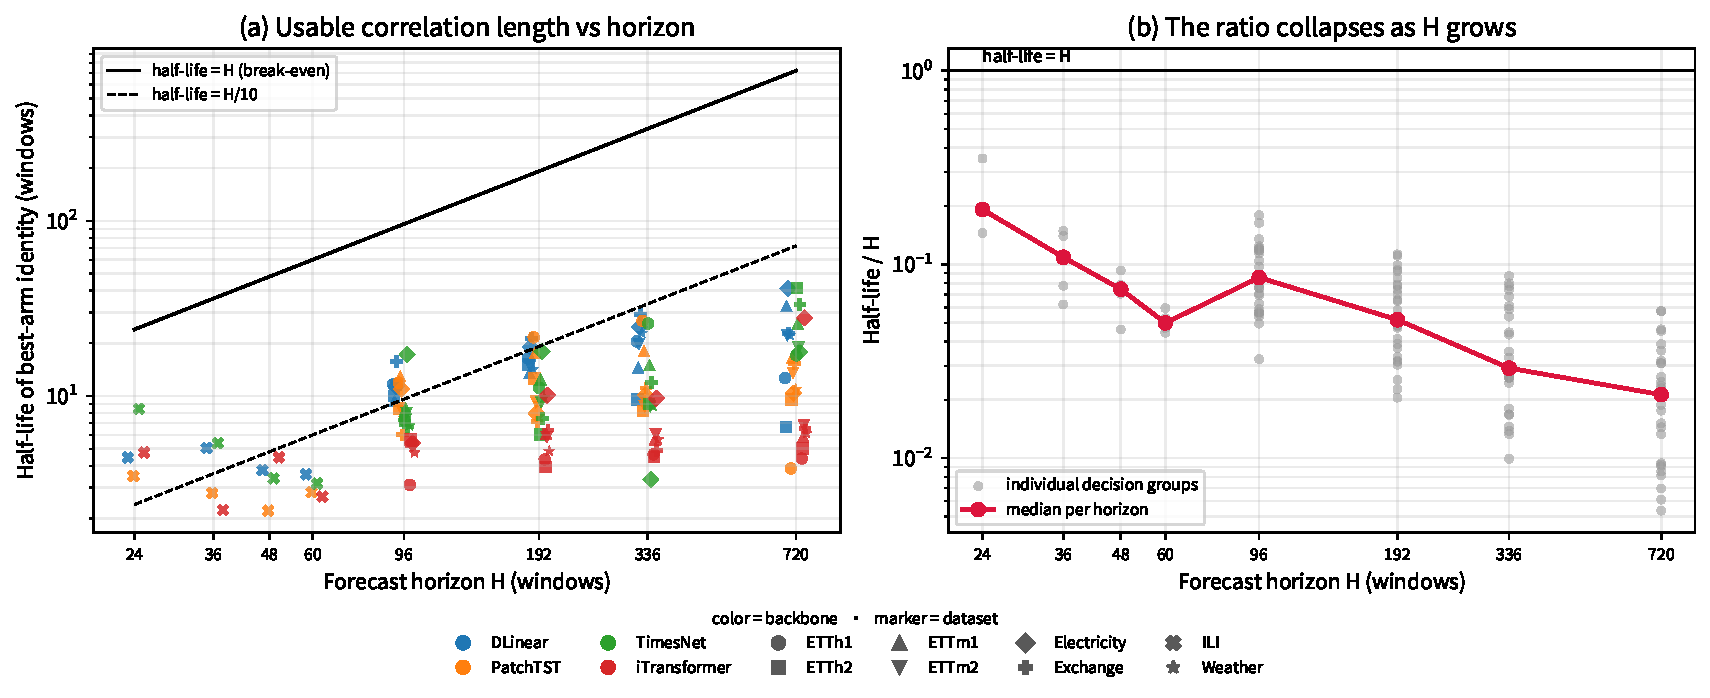
\includegraphics[width=\linewidth]{figs/fig_halflife_vs_horizon.pdf}
\caption{\textbf{The usable correlation length never reaches the decision lag.}
(a) Half-life of best-arm identity vs.\ forecast horizon, one marker per
decision group ($127$; color $=$ backbone, marker $=$ dataset), log--log.
The solid line is the break-even condition half-life $=H$; \emph{no group comes
within an order of magnitude of it}, and most sit below the $H/10$ dashed line.
(b) The ratio half-life$/H$ per horizon: gray dots are groups, red is the median,
falling from $0.19$ at $H{=}24$ to $0.021$ at $H{=}720$. The decline is monotone
\emph{within} each of the two horizon families ($24/36/48/60$ for ILI,
$96/192/336/720$ for the rest); the small step up at $H{=}96$ is the change of
family, not a reversal.}
\label{fig:halflife}
\end{figure}

\begin{figure}[t]
\centering
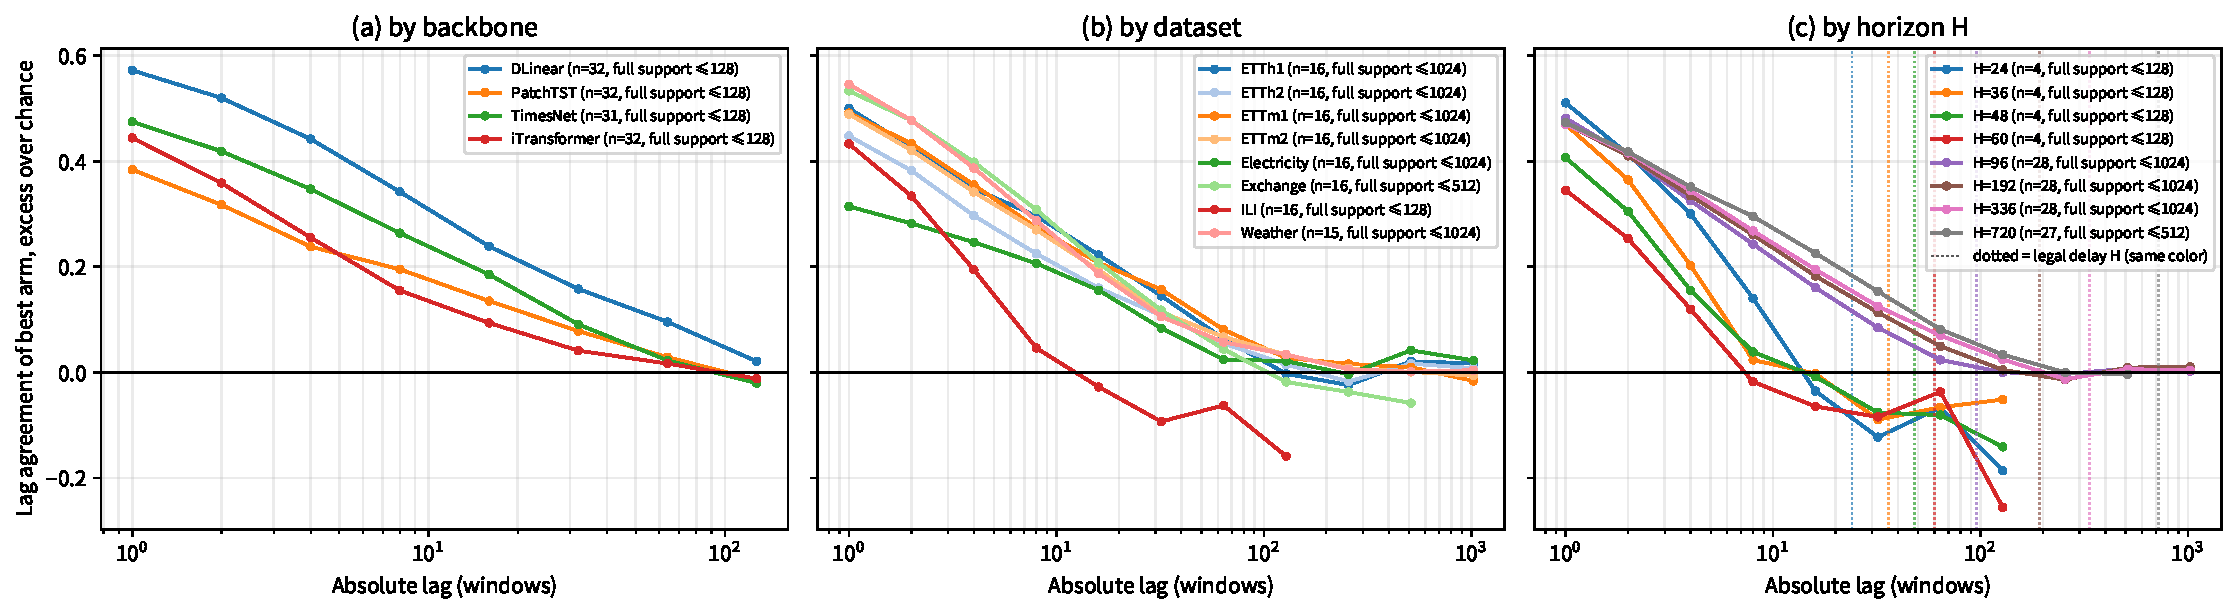
\includegraphics[width=\linewidth]{figs/fig_decay_curves.pdf}
\caption{\textbf{The same decay under three independent stratifications.}
Excess-over-chance agreement of best-arm identity vs.\ absolute lag (windows),
by backbone (a), dataset (b) and horizon (c). Only lags with full support across
the groups in a stratum are drawn. Every curve reaches chance by lag
$\approx10^{2}$; in (c) the dotted vertical lines mark each stratum's legal
decision lag $H$ (same color), and every curve has already flattened at or
before its own line. No stratum is an exception.}
\label{fig:decay}
\end{figure}

\subsection{The headroom is real, just late}
\label{sec:seed}

Proposition~\ref{prop:invariance} is constructive; a skeptic may answer that
real labels are not random permutations. We therefore give a purely empirical
second leg. For $48$ cells we retrain with only the training seed changed
($2021 \to 2022$) and ask how much of the per-window best-arm identity survives.

The key statistic is the \emph{cross-seed oracle}: choose arms with seed A's
per-window $\arg\min$, settle the bill on seed B's errors. It still uses future
information, but only the part of the arm identity that is reproducible, so it
upper-bounds any selector that relies on reproducible structure --- including a
static gate given perfect features.

\begin{table}[t]
\centering\small
\caption{A seed-paired replication shows the per-window structure is real and
largely reproducible, so the failure of every selector cannot be explained as
``there is nothing there to learn''.}
\label{tab:crossseed}
\fitwidth{%
\begin{tabular}{lr}
\toprule
Quantity & Value \\
\midrule
paired cells / seeds & $48$ / $\{2021,2022\}$ \\
same-seed oracle vs.\ best fixed & $+7.26\%$ \\
\textbf{cross-seed oracle (reproducible bound)} & $\mathbf{+5.74\%}$ \\
reproducible share of headroom & $79\%$ \\
cross-seed identity agreement & $0.788$ (chance $0.374$) \\
pairs with $z>2$ & $48/48$ \\
pairs where cross-seed oracle still wins & $46/48$ \\
\midrule
same-arm per-window error correlation & $0.989$ \\
block MSE fluctuation across seeds & $1.33\%$ \\
best fixed arm unchanged across seeds & $88\%$ \\
\bottomrule
\end{tabular}}
\end{table}

The last three rows of Table~\ref{tab:crossseed} are a necessary caveat: if a
backbone converges to the same solution under both seeds, reproducibility is
trivial and the audit has no discriminative power for it (near-convex models such
as \arm{DLinear} are the worst case). With same-arm error correlation $0.989$ and
block-level MSE moving by $1.33\%$, the model does change, yet \emph{which window
wants which plug-in} stays stable. So the finding is not ``there is nothing to
learn'' but the sharper ``the thing to learn is real, and it is unavailable in
time''.

\section{Three selector families, one verdict}
\label{sec:selectors}

We now test the decision problem directly. All numbers are relative to the
deployable \arm{best\_fixed\_val} baseline on identical decision groups.

\subsection{Static complexity-feature gating}
Per window we compute $24$ cheap statistics in five groups --- non-stationarity
(\texttt{w\_ns}), trend and autocorrelation (\texttt{w\_sd}), cross-channel
correlation (\texttt{w\_ch}), spectral concentration (\texttt{w\_fr}) and
predictability/entropy (\texttt{w\_pc}) --- all $O(n\log n)$ from the raw
look-back window, with no access to the target. A gradient-boosted tree is
trained on validation windows (either regressing per-arm gain and thresholding,
or classifying the arm directly) and applied to test windows.

\begin{table}[t]
\centering\small
\caption{Window-level gating. Gains in \% relative to the stated reference;
\arm{bf} = \arm{best\_fixed\_val}. ``in-pool'' trains and applies within each
group; ``LODO'' holds out a whole dataset; ``learnable'' restricts to groups
with $\geq1000$ validation windows.}
\label{tab:gate}
\begin{tabular}{llrrrr}
\toprule
Protocol & head & $N$ & vs \arm{none} & vs \arm{bf} & oracle \\
\midrule
in-pool     & reg & 96 & $+1.50$ & $\mathbf{-0.67}$ & $+9.74$ \\
in-pool     & clf & 96 & $+1.49$ & $-0.65$ & $+9.74$ \\
learnable   & reg & 72 & $+2.46$ & $-0.66$ & $+9.10$ \\
LODO        & reg & 76 & $+1.23$ & $-1.56$ & $+10.46$ \\
\bottomrule
\end{tabular}
\end{table}

Gating loses to a frozen arm by $0.67$ points (positive in $22\%$ of groups,
Wilcoxon signed-rank across groups $p{=}3.1\!\times\!10^{-6}$), captures a
\emph{negative} fraction of the oracle headroom, and its per-window accuracy
($0.416$) is below the majority-class rate ($0.486$). Restricting to
data-rich groups does not help ($-0.66$); requiring cross-dataset transfer makes
it worse ($-1.56$). Stratifying by the number of validation windows
($<200$, $200$--$1000$, $1000$--$5000$, $\geq5000$) gives
$-0.46$, $-1.09$, $-0.60$, $-0.73$: the failure is not a sample-size artifact.
The LODO row covers $76$ of the $96$ gating groups: leaving out one dataset
requires at least three datasets sharing a (backbone, horizon, arm-pool) shape,
which excludes ILI entirely (each ILI horizon exists on one dataset only) and
excludes the four-arm \arm{PatchTST}/\arm{iTransformer} shapes at $H{=}96$ and
$H{=}720$, which span two datasets. The exclusions are structural, not outcome
dependent.

\paragraph{Falsification controls.}
Two controls separate ``window-level information'' from ``switching per se'':
a random switcher matched to the gate's switching frequency and arm marginals
($-1.04$ vs \arm{bf}), and the same model trained on column-shuffled features,
i.e.\ a same-capacity noise-fitting baseline ($-0.54$). The gate's net advantage
is $+0.36$ over random ($66\%$ of groups) and $-0.22$ over shuffled ($26\%$).
The honest reading: after the overfitting baseline is subtracted, the
contribution of window-level features is not distinguishable from zero, and we
do not claim it. Leave-one-group-out feature ablation is consistent --- removing
any of the five feature groups changes the gain by at most $0.13$ points, and
removing the entropy group even \emph{improves} it.

\paragraph{Same-distribution split diagnostic.}
The gate above is trained on validation windows and applied to test windows, so
two confounds remain: validation errors are mildly optimistic (that split also
drives early stopping) and there is a val$\to$test shift. We remove both by
re-running the identical gate \emph{inside a single split}: the first $70\%$ of
windows chronologically to fit, the last $30\%$ to evaluate, with the fixed-arm
baseline \arm{bf\textsubscript{split}} also chosen on the fitting segment, so
neither side sees the evaluation segment. With
\texttt{source}=\arm{val} the optimism is present on both sides and cancels;
with \texttt{source}=\arm{test} the labels have \emph{never} been touched by
early stopping or checkpoint selection, so the label bias is exactly zero and all
backbones are covered. Both are diagnostic upper bounds, not deployable
policies.

\begin{table}[t]
\centering\small
\caption{Same-distribution split diagnostic: gate fitted and evaluated inside one
split (chronological $70/30$), removing both label optimism and val$\to$test
shift. \arm{bf\textsubscript{split}} is the fixed arm chosen on the fitting
segment. Groups with $<200$ fitting or $<100$ evaluation windows are skipped.}
\label{tab:splitgate}
\begin{tabular}{lrrrrr}
\toprule
fit/eval split & $N$ & vs \arm{none} & vs \arm{bf\textsubscript{split}} & win & oracle \\
\midrule
val internal  & $81$  & $+2.01$ & $-1.18$ & $35\%$ & $+11.35$ \\
test internal & $111$ & $+2.33$ & $\mathbf{-0.53}$ & $38\%$ & $+10.37$ \\
\bottomrule
\end{tabular}
\end{table}

The verdict is unchanged (Table~\ref{tab:splitgate}). Under zero drift and zero
label bias the gate still loses to a frozen arm chosen from the same
information ($-0.53$, positive in $38\%$ of groups, $p{=}0.19$), and its
per-window accuracy
($0.411$) is still below the majority-arm rate ($0.486$), beating it in only
$13\%$ of groups. Its share of the $+10.4\%$ oracle headroom is small and, more
importantly, unstably estimated: as a ratio of aggregate means it is
$+2.33/+10.37 = 22\%$, whereas the per-group ratio has median $4.6\%$ and mean
$3.3\%$ with an interquartile range of $-9\%$ to $+35\%$ and a minimum of
$-579\%$, because groups whose oracle headroom is nearly zero put a vanishing
denominator under a noisy numerator. We report all three rather than pick one,
and we do not rest any conclusion on them: the load-bearing fact is the
comparison against the frozen arm, which needs no ratio. This rules out ``the
validation split was used for early
stopping'' and ``val$\to$test shift'' as explanations: what is missing is
window-level signal, not clean labels. One further detail sharpens the main
result: in the test-internal setting the gate is on par with the
\emph{validation}-chosen arm ($+0.08$) while losing to the split-chosen arm
($-0.53$), and the split-chosen arm coincides with the evaluation-segment
argmin in $70\%$ of groups versus $47\%$ in the val-internal setting. The small
gains a window gate appears to make over \arm{best\_fixed\_val} elsewhere are
arm-identity mismatch between splits, not per-window adaptation.

\subsection{Delayed online error feedback}
Static features must transfer across a distribution shift; deployment has a
stronger signal available, namely the \emph{realized} per-arm error on past
windows. We run follow-the-leader over a sliding feedback window of $200$,
with the delay set to exactly $H$ windows, and additionally a no-delay cheating
variant. This is the delayed-feedback regime of~\cite{joulani}, with the
distinguishing feature that the delay is not an implementation nuisance but is
fixed by the forecast horizon itself.

\begin{table}[t]
\centering\small
\caption{Online selection with legal $H$-window delay ($123$ groups). Pool sizes
are nominal; realized arm counts per group are given in \S\ref{sec:protocol}.
``delay cost'' is the no-delay advantage.}
\label{tab:online}
\begin{tabular}{lrrrr}
\toprule
Pool (nominal) & vs \arm{none} & vs \arm{bf} & no-delay & delay cost \\
\midrule
$\leq4$ arms  & $+1.19$ & $\mathbf{-0.87}$ & $+2.47$ & $3.34$\,pp \\
$\leq11$ arms & $+1.31$ & $-0.82$ & $+2.84$ & $3.66$\,pp \\
\bottomrule
\end{tabular}
\end{table}

The legal configuration loses ($-0.87$, positive in $20\%$ of groups) while the
illegal one wins by $+2.47$: a $3.34$-point delay cost. This is the same
conclusion as Table~\ref{tab:persist}, reached with a completely different
estimator and no learned model at all. The count is $123$ of the $127$ decision
groups; the four excluded ones are Exchange at $H{=}720$ on all four backbones,
where the legal delay ($720$ windows) exceeds the number of evaluation windows
($399$), so no legal decision can be made at all. That exclusion is itself an
instance of the thesis, not a limitation of the estimator.

\paragraph{Delay sweep.}
Sweeping the delay in multiples of $H$ (all cells evaluated on one common test
segment, skipping the warm-up of the longest delay --- omitting this dilutes
long-delay rows toward zero and produces the spurious conclusion that $2H$ beats
$1H$) gives a clean break-even point (Table~\ref{tab:delaysweep}).

\begin{table}[t]
\centering\small
\caption{Delay $\times$ feedback-window sweep, gains vs.\ \arm{bf} (\%). ``fb''
is the sliding feedback-window length. Only $\ell\geq1H$ is causally legal.}
\label{tab:delaysweep}
\begin{tabular}{lrrrrl}
\toprule
delay & fb$=50$ & $200$ & $1000$ & $3000$ & legal? \\
\midrule
$0$      & $+4.59$ & $+2.19$ & $+0.96$ & $+0.88$ & cheat \\
$0.25H$  & $+0.83$ & $+0.07$ & $+0.22$ & $+0.43$ & cheat \\
$0.5H$   & $-0.49$ & $-0.64$ & $+0.01$ & $+0.32$ & cheat \\
$\mathbf{1H}$ & $-1.36$ & $-0.77$ & $-0.13$ & $+0.12$ & \textbf{yes} \\
$2H$     & $-0.92$ & $-0.61$ & $-0.01$ & $+0.22$ & yes \\
\bottomrule
\end{tabular}
\end{table}

Averaged over feedback windows on the $103$ groups with common support, the
break-even delay is $\mathbf{0.25\times H}$: at $1\times H$ the policy is
$-0.38\%$, at zero delay $+1.89\%$. Note also the interaction: short feedback
windows are best when the delay is small and worst when it is legal, because
adaptation speed is only useful if the information is fresh.

\subsection{Horizon-aware checkpoint selection}
The third family is zero-compute: instead of selecting the checkpoint by overall
validation MSE, we select it by a horizon-aware read of the same training logs
(worst forecast segment, long-segment MSE, slope-penalized, rank aggregation,
last epoch). Over all $844$ cells, none beats the validation-MSE baseline
(gains $-0.002$ to $-0.074$; taking the last epoch is $-2.03$,
$p{=}6.8\!\times\!10^{-13}$), while the post-hoc oracle checkpoint would give
$+0.92$. Even re-reading existing logs yields nothing.

\section{What is actually recoverable}
\label{sec:recover}

If online feedback loses to \arm{best\_fixed\_val}, what did its $+1.19\%$ over
\arm{none} consist of? Decomposing against the post-hoc constant arm
\arm{best\_fixed\_test} settles it (Table~\ref{tab:decomp}).

\begin{table}[t]
\centering\small
\caption{Decomposition of the online policy's gain over \arm{none}. The
time-varying component is negative; the whole effect is the correction of a
constant mis-selection.}
\label{tab:decomp}
\begin{tabular}{lr}
\toprule
Component & Value \\
\midrule
$\arm{bf\_test} - \arm{bf\_val}$ & $+1.36\%$ \\
\quad (groups where val picks the wrong arm) & $34\%$ \\
$\arm{online} - \arm{bf\_test}$ & $-2.32\%$ \\
\quad (groups where this is positive) & $5\%$ \\
\bottomrule
\end{tabular}
\end{table}

The time-varying component is negative. The only real effect is that
validation-based arm choice is wrong in a third of groups, and delayed feedback
partially corrects that \emph{constant} choice. This is a legitimate, modest,
deployable claim: \emph{use online feedback to fix plug-in mis-selection, not to
adapt per window.} Any paper claiming window-level adaptation must publish the
\arm{best\_fixed\_test} column, or the claim is unfalsifiable.

\section{A checklist for adaptive-selection claims}
\label{sec:checklist}

The audit generalizes beyond plug-ins to any ``learn which model/module to use
when'' claim. We propose five tests, all cheap once per-window errors are
persisted:

\begin{enumerate}\itemsep2pt
\item \textbf{Re-labeling test.} Recompute your oracle after permuting arm
labels independently per window. If it does not move
(Prop.~\ref{prop:invariance}), it is not evidence of learnability and must not
be cited as headroom.
\item \textbf{Correlation-length test.} Report the half-life of best-arm
identity in units of the decision lag. If $\text{half-life}/\text{lag} \ll 1$
(here: mean $0.061$, median $0.051$), no causal selector can work; ours is
$<0.25$ in $20/20$ strata.
\item \textbf{Deployable-baseline test.} Compare against the arm frozen from
validation, and publish the post-hoc constant arm too, so that
``adaptation'' is separated from ``fixing a bad constant choice''
(\S\ref{sec:recover}).
\item \textbf{Shuffled-feature test.} Train the identical model on
column-shuffled features. The difference, not the raw gain, is your evidence
(here: $-0.22$ points).
\item \textbf{Same-split test.} Before blaming distribution shift or noisy
labels, fit and evaluate the selector inside one split, chronologically, with
the fixed-arm baseline chosen on the same fitting segment. A selector that
cannot win with zero drift and unbiased labels
(Table~\ref{tab:splitgate}) will not win in deployment, and this costs no
additional training.
\end{enumerate}

Tests 1--2 say whether the target is reachable, test 5 whether the pipeline is
to blame, tests 3--4 whether a reported win is a win.

For the reporting side, \S\ref{sec:main}--\S\ref{sec:effectsize} add four more
that cost nothing but a few lines of analysis code:
aggregate with pairwise dropping and publish the per-arm block counts;
report every verdict on at least two error metrics, since one of our three arms
changes verdict between MSE and MAE;
report the median, the mean and the tail fractions together, because the first
two disagree in sign for one of our arms and the tail is where the deployment
risk lives;
and put the effect next to the run-to-run noise of a training seed and next to
the wall-clock time it costs, because $28\%$ of our block-level effects are inside
seed noise and the arm with the largest compute surcharge is the one that hurts
most. Finally, report any plug-in both at its published default and per-cell
tuned, with the gap stated (\S\ref{sec:tuning}).

\section{Threats to validity}
\label{sec:threats}

\paragraph{A provenance bug we found in ourselves.}
An earlier version of this study trained the window gate on validation error
traces whose order had been permuted by a shuffling data loader (the library
disables shuffling for \texttt{test} but not for \texttt{val}). Features of
window $i$ were paired with the error of a random window $j$. Every
gating/control/ablation number was therefore invalid, while all test-side audits
were unaffected (the test loader never shuffles) and all per-arm \emph{means}
were unaffected (a mean is permutation-invariant, so
\arm{best\_fixed\_val} survived). We re-ran $328$ cells, added a machine-checked
provenance marker asserting deterministic loader order, and made the analysis
code refuse unmarked arrays rather than silently reuse them. We report this
because the corrected gating number ($-0.67$) is smaller in magnitude than the
buggy one ($-1.76$): the bug was making our negative result look stronger than
it is.

\paragraph{Coverage asymmetry.}
The test-side audits (Tables~\ref{tab:persist}, \ref{tab:online}) use $127$
decision groups; only $96$ have a certified deterministic validation window order
and can therefore train a gate (Table~\ref{tab:gate}). Table~\ref{tab:coverage}
makes the gap explicit rather than asserting it is harmless. All $31$ missing
groups are \arm{TimesNet}, for a bookkeeping reason: those validation traces
predate the provenance marker above. The question is whether they differ on the
quantities that decide learnability. They do not: half-life over the legal delay
is $0.053$ versus $0.049$ for covered groups, and excess above chance at delay
$H$ is $-0.002$ versus $-0.008$ --- the same distribution, both far from the
threshold at which per-window selection could pay. The missing groups have a
\emph{larger} oracle headroom ($+11.4$ vs $+9.7$), which is precisely the
direction that would make gating look good if headroom were the operative
variable; it is not. Filling the gap would add samples, not reverse the sign.
Two independent audits also cover all four backbones including \arm{TimesNet}
and reach the same verdict: the test-internal split diagnostic
(Table~\ref{tab:splitgate}, $-0.53$ there) and the lead-time audit of
\S\ref{sec:leadtime}, which uses all $128$ blocks.

\begin{table}[t]
\centering\small
\caption{Explicit coverage gap between the test-side audits and the
gating protocols, with the audit statistics that decide learnability.
$t_{1/2}/H$ is the median arm-identity half-life divided by the legal feedback
delay; exc@$H$ is the mean excess above chance at delay $H$.}
\label{tab:coverage}
\begin{tabular}{lrrrrr}
\toprule
backbone & audit & gate & oracle & $t_{1/2}/H$ & exc@$H$ \\
\midrule
DLinear      & $32$ & $32$ & $+14.73$ & $0.076$ & $-0.010$ \\
PatchTST     & $32$ & $32$ & $+4.66$  & $0.047$ & $-0.010$ \\
iTransformer & $32$ & $32$ & $+9.83$  & $0.030$ & $-0.005$ \\
TimesNet     & $31$ & $0$  & $+11.40$ & $0.053$ & $-0.002$ \\
\midrule
covered      & $96$ & $96$ & $+9.74$  & $0.049$ & $-0.008$ \\
missing      & $31$ & $0$  & $+11.40$ & $0.053$ & $-0.002$ \\
\bottomrule
\end{tabular}
\end{table}

\paragraph{Other caveats.}
(i) A small number of windows produce NaN features when a channel is constant
inside the window; the tree model handles missing values natively and we do not
impute. (ii) \arm{san\_lite} is a training-free surrogate, not the original
method, and the compute surcharge we report in \S\ref{sec:effectsize} is that of
the surrogate. (iii) The $\alpha{=}0.5$ reference comes from phase 1/2, not the
sweep; we aligned seeds and checked the reproducibility of duplicate cells.
(iv) Missing cells concentrate in the expensive corner, so every cross-backbone
average in this paper is computed on a single common block set.
(v) The lead-time audit of \S\ref{sec:leadtime} resolves the horizon into
quarters, not individual steps; a finer partition could expose switching that
quarters average away, though it cannot raise the oracle ceiling by much, since
the quarter-level oracle is already within $0.24\%$ of a frozen arm.
(vi) \arm{revin} was deliberately pruned outside \arm{DLinear}
(\S\ref{sec:protocol}), so its metric-level verdict in
Table~\ref{tab:metric-robust} rests on $44$ blocks that are predominantly one
backbone, and we do not generalize it; the $12$-cell verification subset supports
the no-op prediction but is too small to support a metric-level claim.
(vii) All conclusions are for the four backbones and eight datasets studied at
look-back $96$ ($36$ for ILI); zero-shot foundation models are out of scope
(they require bf16, unavailable on the target hardware, and would introduce an
incomparable baseline).

\section{Conclusions}

Plug-in gains for time series forecasting are strongly conditional --- the same
frequency-domain loss moves a linear backbone by $+4.6\%$ and a patch
transformer by $-16.6\%$ --- and the way the community aggregates, measures,
summarizes and tunes them inflates the reported effect past the effect itself:
block filtering, the metric, the choice of mean or median, and the default
hyper-parameter each move the headline by more than the claim. That
conditionality invites a selector, and a per-window oracle appears to promise
$10\%$ for building one. We showed that this promise is a statistical mirage
(the oracle is invariant to per-window arm re-labeling), that the underlying
structure is nonetheless real and reproducible across training seeds, and that
it is unusable anyway because the identity of the best arm decorrelates with a
median half-life of $5.1\%$ of the forecast horizon (mean $6.1\%$) while
deployment forces a decision lag of exactly one horizon. Three selector families
fail accordingly and
the break-even delay is a quarter of a horizon. The one selection axis that
deployment does \emph{not} forbid, the lead-time index, turns out to have an
oracle headroom of $+0.24\%$, so it is closed for the opposite reason. The only
recoverable gain is the correction of a constant mis-selection. We recommend that
the field stop tuning gates and start publishing the audits above.

% CRediT is emitted from the \credit{} declaration in the front matter; do not
% also write the section out by hand or it appears twice.
\printcredits

\section*{Declaration of competing interest}
The authors declare that they have no known competing financial interests or
personal relationships that could have appeared to influence the work reported in
this paper.

\section*{Funding}
This research did not receive any specific grant from funding agencies in the
public, commercial, or not-for-profit sectors.

\section*{Declaration of generative AI and AI-assisted technologies in the
writing process}
During the preparation of this work the authors used a large language model to
assist with copy-editing, LaTeX formatting and the drafting of analysis and
plotting scripts. All experimental design, statistical decisions, numerical
results and scientific conclusions were produced and verified by the authors, who
take full responsibility for the content of the publication.

\section*{Relation to other work by the authors}
This study and the companion manuscript \citep{companion2026b} share an
experimental infrastructure and a research programme but address disjoint
questions and report disjoint results: this paper asks whether per-window plug-in
selection is learnable under a legal feedback delay, and the companion asks
whether a stored per-sample artifact is in the order its consumer assumes.
Neither manuscript's claims depend on the other's; the overlap is disclosed here
so that editors and reviewers can assess it directly.

\section*{Data availability}
All datasets used in this study are public standard benchmarks (ETT, Electricity,
Exchange, Weather, ILI) and are not redistributed here. The artifacts required to
recompute every number in this paper are released at
\url{https://github.com/oscarliu2019/plugin-selection-audit}: the experiment
configurations; per-run result tables for the $844$ phase-1 and $423$ phase-2
runs; per-block aggregates for the $768$ phase-3 runs of the $\alpha$ sweep; the
window-level feature table; the per-group outputs of every audit reported here
(decay curves and half-lives, oracle re-labeling, delayed-feedback and lead-time
sweeps, seed replication, split diagnostics, coverage gap); and the audit,
statistics, table and figure generators. The raw per-window error arrays written
during training are not redistributed; they are regenerated by re-running the
phase-2 configuration with the \texttt{-{}-save-window-mse} flag. Each table
states the artifact it is regenerated from, and the commands are listed in the
repository \texttt{README}. A verification script,
\texttt{tools/verify\_paper\_numbers.py}, re-derives every quantitative claim in
this manuscript from those artifacts and fails on any mismatch; it prints the
claim identifier, the section, the value printed here and the value recomputed.

% >>> Software Heritage archive (generated by tools/set_metadata.py)
\begin{sloppypar}
The repository is also archived permanently in Software Heritage: the revision
from which this manuscript was produced is
\texttt{swh:1:rev:ec90998cd56de249ab48eb381934a93a82d3e12a} (origin
\url{https://github.com/oscarliu2019/plugin-selection-audit}, visit \texttt{swh:1:snp:cd0b09f87d11cd06b53af22f6b0439fd8687a009}).
\end{sloppypar}
% <<< Software Heritage archive


% >>> archive DOI (generated by tools/set_metadata.py)
The exact release from which every number in this manuscript was computed is
archived, with all artifacts, at \url{https://doi.org/10.5281/zenodo.22809153} (DOI: \texttt{10.5281/zenodo.22809153}); the
repository above is its development mirror.
% <<< archive DOI

\bibliographystyle{elsarticle-num}
\bibliography{refs}

\end{document}
